\chapter{Estatística Descritiva}

Neste capítulo da apostila, vamos explorar o passo a passo de como realizar análises de estatística descritiva no Jamovi. Aprenderemos como utilizar as diversas ferramentas disponíveis no software para organizar, resumir e apresentar os dados de maneira clara e concisa.

No capítulo anterior nós aprendemos como importar os dados para o Jamovi, seja através da importação de arquivos ou inserção direta na planilha. Em seguida, abordaremos as principais medidas de tendência central, como média, mediana e moda, e as medidas de dispersão, como desvio padrão, variância e amplitude. Você aprenderá como calcular essas medidas usando o Jamovi e interpretar os resultados.

Em seguida, mergulharemos nos recursos de visualização de dados do Jamovi. Exploraremos os diversos gráficos disponíveis, como gráficos de barras, gráficos de dispersão, gráficos de linha, gráficos de boxplot e histogramas. Você aprenderá como criar esses gráficos, personalizá-los e interpretar as informações que eles fornecem sobre seus dados.

Continuaremos com a criação de tabelas de frequência, que mostrarão a distribuição dos dados em categorias ou intervalos. Você aprenderá a criar tabelas de frequência no Jamovi e interpretar os resultados para entender a distribuição dos seus dados.

Em seguida, exploraremos as tabelas cruzadas, uma técnica poderosa para analisar a relação entre duas ou mais variáveis. Aprenderemos como criar tabelas cruzadas no Jamovi e interpretar os resultados para identificar associações ou padrões entre as variáveis.

Por fim, abordaremos a criação de relatórios de estatísticas descritivas no Jamovi. Você aprenderá como criar relatórios que resumem suas análises, incluindo informações sobre as medidas calculadas, gráficos relevantes e interpretação dos resultados. Esses relatórios serão úteis para compartilhar seus resultados com outros pesquisadores ou colaboradores.

Ao final deste capítulo, você terá adquirido as habilidades necessárias para realizar análises de estatística descritiva no Jamovi. Você estará apto a utilizar as diversas ferramentas e recursos oferecidos pelo software para explorar e descrever seus dados de forma eficiente e precisa. A estatística descritiva no Jamovi será uma poderosa aliada em suas análises e na comunicação clara dos resultados obtidos.

A estatística descritiva é uma parte fundamental da análise de dados, pois oferece uma visão geral e resumida das características dos dados. No Jamovi, um software estatístico de código aberto e amigável, você pode encontrar várias ferramentas e recursos para realizar estatística descritiva de maneira eficiente.

Ao utilizar o Jamovi, você pode importar seus dados ou inseri-los diretamente na planilha. Em seguida, você pode explorar as diversas opções disponíveis para realizar análises descritivas. Alguns dos recursos mais comuns incluem:

\begin{itemize}
    \item Medidas de tendência central: O Jamovi oferece várias opções para calcular medidas de tendência central, como média, mediana e moda. Essas medidas ajudam a identificar valores centrais ou típicos em seus dados.
    \item Medidas de dispersão: Além das medidas de tendência central, o Jamovi também permite calcular medidas de dispersão, como desvio padrão, variância e amplitude. Essas medidas fornecem informações sobre a variação ou dispersão dos seus dados.
    \item Gráficos: O Jamovi possui uma ampla variedade de gráficos disponíveis para visualizar seus dados de forma clara e compreensível. Você pode criar gráficos de barras, gráficos de dispersão, gráficos de linha, gráficos de boxplot, histogramas, entre outros. Esses gráficos podem ajudar a identificar padrões, tendências e outliers nos seus dados.
    \item Tabelas de frequência: O Jamovi permite criar tabelas de frequência, que mostram a distribuição dos seus dados em categorias ou intervalos. Essas tabelas são úteis para identificar a frequência de ocorrência de valores específicos ou a distribuição dos seus dados em diferentes categorias.
    \item Tabelas cruzadas: Com o Jamovi, você pode criar tabelas cruzadas para explorar a relação entre duas ou mais variáveis. Isso permite analisar como as diferentes variáveis estão relacionadas entre si e identificar possíveis associações ou padrões.
    \item Relatórios: O Jamovi oferece a opção de criar relatórios de estatísticas descritivas para compartilhar com outros pesquisadores ou colaboradores. Esses relatórios podem incluir informações sobre as análises realizadas, resultados obtidos e gráficos relevantes, facilitando a comunicação dos resultados de forma clara e concisa.
\end{itemize}

Além desses recursos, o Jamovi também oferece suporte a uma ampla gama de técnicas estatísticas avançadas, como testes de hipóteses, análise de variância (ANOVA), regressão, análise fatorial e muito mais. Com sua interface intuitiva e recursos poderosos, o Jamovi é uma ferramenta acessível e eficiente para realizar análises estatísticas descritivas.

\section{Medidas de tendência central}


As medidas de tendência central são estatísticas utilizadas na análise descritiva para resumir e descrever um conjunto de dados, fornecendo uma medida representativa do centro dos valores observados. Essas medidas são úteis para entender as características e propriedades centrais dos dados, permitindo uma compreensão mais clara e concisa da distribuição dos valores.

\subsection{Média}

A média é uma medida de tendência central amplamente utilizada na estatística descritiva. É calculada como a soma de todos os valores em um conjunto de dados dividida pelo número de observações. A média é frequentemente utilizada para determinar um valor típico ou representativo de um conjunto de dados.

A média é uma medida robusta, pois leva em consideração todos os valores do conjunto de dados. Ela é especialmente útil quando os dados estão distribuídos de forma relativamente simétrica e não possuem valores extremos significativos. No entanto, é importante ter cuidado ao usar a média quando há valores discrepantes ou uma distribuição assimétrica, pois esses casos podem distorcer a interpretação dos resultados.

A média é fácil de calcular e fornece uma representação numérica única para resumir os dados. Ela possui propriedades matemáticas úteis, como a propriedade de preservar a soma (a soma das médias é igual à média das somas) e pode ser usada para comparar conjuntos de dados diferentes.

\[
\bar{x} = \frac{1}{n} \sum_{i=1}^{n} x_i
\]

Ao interpretar a média, é importante considerar o contexto do problema em questão. Ela pode ser utilizada para compreender características centrais de um conjunto de dados, como a média de salários de uma população, a média de notas de um grupo de estudantes ou a média de idades de um determinado grupo.

No entanto, é fundamental lembrar que a média não fornece informações sobre a dispersão ou variabilidade dos dados. Portanto, é sempre recomendado complementar a análise com outras medidas descritivas, como o desvio padrão, para ter uma compreensão completa da distribuição dos dados.

Para calcular a média no Jamovi, você pode seguir as etapas abaixo:

\begin{enumerate}
    \item Importe seus dados ou insira-os diretamente na planilha do Jamovi. Certifique-se de que os dados estejam organizados em uma única coluna ou em várias colunas, dependendo da sua estrutura.
    \item Selecione a coluna que contém os dados dos quais você deseja calcular a média. Para fazer isso, clique no cabeçalho da coluna ou arraste o mouse para selecionar várias colunas.
    \item No painel de Análises, localizado à direita da tela, clique na seção "Descriptive Statistics" (Estatísticas Descritivas).
    \item Na seção de estatísticas descritivas, você encontrará várias opções. Procure por "Mean" (Média) e marque a caixa ao lado dela.
    \item Assim que você marcar a caixa de seleção "Mean" (Média), o Jamovi calculará automaticamente a média para os dados selecionados. O valor da média será exibido na tabela de resultados.
    \item Se você deseja realizar o cálculo da média para grupos específicos de dados, você pode utilizar a função de agrupamento. Para isso, clique no ícone "Group by" (Agrupar por) no painel de estatísticas descritivas. Selecione a variável que contém os grupos ou categorias e o Jamovi calculará as médias separadamente para cada grupo.
    \item Para visualizar os resultados de forma mais clara, você pode criar um gráfico de barras ou um gráfico de linha que exiba as médias para cada grupo. Para isso, clique na seção "Visualize" (Visualizar) no painel de estatísticas descritivas e escolha o tipo de gráfico que melhor se adequa aos seus dados.
\end{enumerate}

\subsection{Moda}

A moda é uma medida de tendência central na estatística descritiva que representa o valor ou valores que ocorrem com maior frequência em um conjunto de dados. Em outras palavras, a moda indica o valor mais comum ou popular em um conjunto de observações.

Ao contrário da média, que é calculada a partir da soma de todos os valores dividida pelo número de observações, a moda é determinada pela identificação do valor ou valores que aparecem com maior frequência. Pode haver um único valor de moda, conhecido como moda unimodal, ou pode haver mais de um valor de moda, chamado de moda bimodal, trimodal ou multimodal.

A moda é especialmente útil quando se lida com dados categóricos ou discretos, como categorias de produtos, cores favoritas, resultados de votações, entre outros. Ela também pode ser aplicada a dados contínuos, embora seja menos comum nesse contexto.

A moda é uma medida relativamente fácil de calcular, uma vez que envolve apenas a contagem dos valores e a identificação do valor mais frequente. No entanto, assim como a média, a moda pode não ser suficiente para descrever completamente a distribuição dos dados. Por exemplo, em um conjunto de dados em que todos os valores ocorrem apenas uma vez, não haverá um valor de moda claro.

É importante observar que, ao contrário da média e da mediana, a moda não é afetada por valores extremos ou discrepantes, pois seu cálculo é baseado na frequência de ocorrência dos valores. Isso faz com que a moda seja uma medida robusta em relação a valores atípicos.

No Jamovi, calcular a moda pode ser feito seguindo este passo a passo:

\begin{enumerate}
    \item Importe seus dados ou insira-os diretamente na planilha do Jamovi. Certifique-se de que os dados estejam organizados em uma única coluna ou em várias colunas, dependendo da sua estrutura.
    \item Selecione a coluna que contém os dados dos quais você deseja calcular a moda. Para fazer isso, clique no cabeçalho da coluna ou arraste o mouse para selecionar várias colunas.
    \item No painel de Análises, localizado à direita da tela, clique na seção "Descriptive Statistics" (Estatísticas Descritivas).
    \item Na seção de estatísticas descritivas, você encontrará várias opções. Procure por "Mode" (Moda) e marque a caixa ao lado dela.
    \item Assim que você marcar a caixa de seleção "Mode" (Moda), o Jamovi calculará automaticamente a moda para os dados selecionados. O valor ou valores da moda serão exibidos na tabela de resultados.
    \item Se você deseja calcular a moda para grupos específicos de dados, utilize a função de agrupamento. Clique no ícone "Group by" (Agrupar por) no painel de estatísticas descritivas. Selecione a variável que contém os grupos ou categorias, e o Jamovi calculará as modas separadamente para cada grupo.
    \item Caso o conjunto de dados não apresente um valor de moda claro (todos os valores ocorrem apenas uma vez ou não há valores que se repitam com maior frequência), o Jamovi indicará a ausência de moda na tabela de resultados.
\end{enumerate}

\[
\text{moda} = \text{valor mais frequente na amostra}
\]

\subsection{Mediana}

Suponha que temos a seguinte lista de números: $2, 3, 5, 7, 8, 10, 12$. Para encontrar a mediana, primeiro precisamos ordenar a lista em ordem crescente: $2, 3, 5, 7, 8, 10, 12$. Em seguida, encontramos o valor do meio da lista, que é $7$. Portanto, a mediana desta lista é $7$.

Podemos representar a mediana graficamente usando um histograma. O valor da mediana é o ponto em que a curva do histograma é dividida em duas partes iguais. Veja o exemplo abaixo:

\begin{center}
    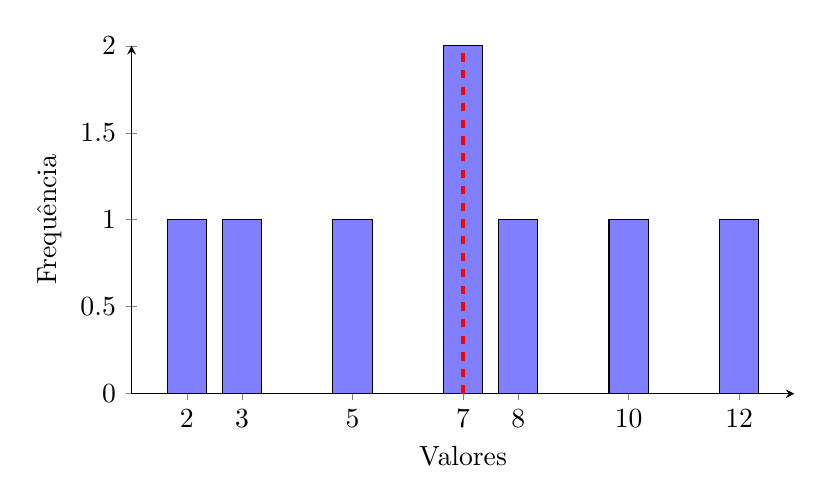
\begin{tikzpicture}
    \begin{axis}[
    ybar,
    ymin=0,
    ymax=2,
    bar width=0.5cm, 
    xtick=data,
    xticklabels={$2$,$3$,$5$,$7$,$8$,$10$,$12$},
    xlabel=Valores,
    ylabel=Frequência,
    width=10cm,
    height=6cm,
    axis lines=left,
    enlarge x limits=0.1,
    enlarge y limits=0,
    clip=false
    ]
    \addplot[fill=blue!50] coordinates {
    (2,1) (3,1) (5,1) (7,2) (8,1) (10,1) (12,1)
    };
    \draw[dashed] (axis cs:7,0) -- (axis cs:7,2);
    \draw[red, dashed, ultra thick] (axis cs:7,0) -- (axis cs:7,2);
    \end{axis}
    \end{tikzpicture}
\end{center}

Neste exemplo, a mediana é $7$, que é o ponto em que a curva do histograma é dividida em duas partes iguais.

Note que, se a lista tivesse um número par de elementos, a mediana seria a média dos dois valores do meio. Por exemplo, se a lista fosse $2, 3, 5, 7, 8, 10$, a mediana seria $(5+7)/2 = 6$.

\section{Medidas de Dispersão}

\subsection{Desvio Padrão}

O desvio padrão é uma medida estatística que indica a dispersão ou variabilidade dos valores em relação à média de um conjunto de dados. Ele fornece uma medida da diferença média entre cada valor e a média do conjunto de dados.

O desvio padrão é calculado em duas etapas principais: primeiro, calcula-se a diferença entre cada valor e a média; em seguida, essas diferenças são somadas, elevadas ao quadrado, e a média desses quadrados é calculada. A raiz quadrada dessa média é o desvio padrão.

\[
s = \sqrt{\frac{1}{n-1} \sum_{i=1}^{n} (x_i - \bar{x})^2}
\]

Uma interpretação do desvio padrão é que ele mede o quanto os valores se afastam, em média, da média. Quanto maior o desvio padrão, maior é a dispersão dos valores em relação à média. Por outro lado, um desvio padrão menor indica que os valores estão mais próximos da média.

O desvio padrão é uma medida importante para entender a variabilidade e a consistência dos dados. Ele pode ajudar a identificar se os valores estão agrupados ou se estão mais dispersos. Além disso, o desvio padrão é usado em muitas outras técnicas estatísticas, como a inferência estatística, para avaliar a precisão das estimativas.

É importante lembrar que o desvio padrão é sensível a valores extremos, pois eles podem influenciar significativamente a medida. Portanto, é essencial considerar o contexto dos dados e interpretar o desvio padrão em conjunto com outras medidas descritivas, como a média e a mediana, para obter uma visão completa da distribuição dos dados.

No Jamovi, calcular o desvio padrão pode ser feito seguindo este passo a passo:

\begin{enumerate}
    \item Importe seus dados ou insira-os diretamente na planilha do Jamovi. Certifique-se de que os dados estejam organizados em uma única coluna ou em várias colunas, dependendo da sua estrutura.
    \item Selecione a coluna que contém os dados dos quais você deseja calcular o desvio padrão. Para fazer isso, clique no cabeçalho da coluna ou arraste o mouse para selecionar várias colunas.
    \item No painel de Análises, localizado à direita da tela, clique na seção "Descriptive Statistics" (Estatísticas Descritivas).
    \item Na seção de estatísticas descritivas, você encontrará várias opções. Procure por "Standard Deviation" (Desvio Padrão) e marque a caixa ao lado dela.
    \item Assim que você marcar a caixa de seleção "Standard Deviation" (Desvio Padrão), o Jamovi calculará automaticamente o desvio padrão para os dados selecionados. O valor do desvio padrão será exibido na tabela de resultados.
    \item Se você deseja calcular o desvio padrão para grupos específicos de dados, utilize a função de agrupamento. Clique no ícone "Group by" (Agrupar por) no painel de estatísticas descritivas. Selecione a variável que contém os grupos ou categorias, e o Jamovi calculará os desvios padrão separadamente para cada grupo.
    \item O Jamovi também oferece a opção de calcular outros tipos de desvio padrão, como o desvio padrão populacional. Para isso, clique no ícone de configurações ao lado da opção "Standard Deviation" (Desvio Padrão) e selecione a opção desejada.
\end{enumerate}